\documentclass[a4paper, 12pt]{article}
\usepackage[utf8]{inputenc}
\usepackage{geometry}
\usepackage{setspace}
\usepackage{amsmath} 
\usepackage{lscape}
\usepackage{graphicx}
\usepackage[affil-it]{authblk}
\usepackage{apacite}
%\usepackage[notes,backend=biber]{biblatex-chicago}

%\bibliography{bib}
\geometry{margin=1in}
\doublespacing



\begin{document}
\title{Presidents, Polarization and the U.S. Economy}
\author{Evin Tunador\thanks{Thank you to Dr. Vipul Bhatt, Dr. Robert Stauffer and Julian Gouffray  for the helpful feedback.}}
%\affil{James Madison University}
\date{December 2020}

\maketitle



\begin{abstract}
    For decades there has been a discrepancy in economic performance between U.S. presidents, with Democrats having the edge in a multitude of cases including real GDP growth, the focus of this paper. \citeA{blinderwatson2016} utilized a Vector Autoregression (VAR) model with an array of economic indicators to account for this gap. This paper extends their analysis through a data update and the inclusion of an index for political polarization. The gap in economic performance is heavily mitigated by the relatively small increase in sample size from adding the post-2012 data of Obama’s second and most of Trump’s term. Also of note is the finding that increased polarization predicts positive GDP growth which contradicts theory and previous research. Finally, the following facts all together strongly point towards polarization being a mediating factor of the discrepancy: (I) polarization is higher when a Democrat is president, (II) its inclusion decreases the predictive power of presidential party on GDP growth, (III) it has some predictive power on presidential party and (IV) it is the best predictor of GDP growth in the analysis. However, the lack of data on polarization during the pre-Reagan years limits this conclusion.
\end{abstract}


\newpage
\section{Introduction}
\setlength{\parindent}{7ex}
Despite the common conception of Republicans as being the party of the economy, for decades the United States has seen lower real GDP growth rates while a Republican holds the office of president. This disparity will henceforth be referred to as the “D-R gap.” The purpose of this paper is to explain said gap, with contributions consisting of both a data update to previous research and the inclusion of an index for political polarization. Theoretically, positive shocks to polarization should raise fiscal policy volatility, thereby hampering growth due to increased economic uncertainty \cite{azzimontiTalbert2014, bakerBloomDavis2016}. Key to this analysis is the question of whether presidents of differing parties experienced unequal amounts of polarization and if said potential disparity can help account for the D-R gap. \par 

The most significant finding is that the addition of Obama's second term and most of Trump's (2013:Q2 to 2020:Q2) heavily mitigates the D-R gap. Second is that political polarization is the strongest explanatory variable for the sample period in which data was available and that increased polarization predicts an increase in GDP growth rate. This contradicts theory and previous research and potential explanations are discussed in Section 6. Although beyond the scope of this analysis and in need of further research before conclusions may be drawn, the predictive strength is likely attributable to some as-of-yet unexplored byproduct of polarization rather than being a direct effect of polarization onto the economy. Finally, various results also indicate that polarization may be a mediating factor of the D-R gap, but this finding is limited by the variable's restricted sample size. \par

Section 2 of this paper continues the discussion of the relevant literature on the subject. Section 3 details the variables that have been selected for use in this analysis. Section 4 explains the methodology of the Vector Autoregression (VAR) model utilized, 5 the results and 6 acts as a conclusion. 



\section{Related Literature}

\citeA{blinderwatson2016} found a D-R gap of 1.79 percentage points within their sample going from Truman’s second term through Obama’s first (1949:Q2 to 2013:Q1) before controlling for a variety of potential explanations. For some theorized predictors they used multiple data-sets, models, and/or formats and tested which had the most explanatory power before deciding to include the winner. Rather than repeat this process, only their top choices have been included in this paper for sake of brevity. Which party controlled congress and whether there was agreement between branches had an insignificant lean towards Democrats and agreement. Other insignificant factors they analyzed include trends, initial conditions including inheriting recessions, fiscal policy and consumer confidence. Also of note are financial sector disruptions and interest rates which \citeauthor{blinderwatson2016} did not find to be significant but have still been included in this analysis thanks to increased relevance gained by the data update. Foreign growth is the only variable they found to be significant that is not explored in this paper because of unavailability for the full sampling period of Model 1. The variables with the strongest explanatory power were oil price shocks, total factor productivity, and defense spending specifically from the Korean war. \citeauthor{blinderwatson2016}'s best model accounted for a bit over half of the observed D-R gap. \par

The final variable of interest to this analysis is political polarization at the federal level. As can be seen in Figure 1, since the 1980s the ideological viewpoints of the United States' two political parties have diverged and become more concentrated around their respective means\cite{mccarty2006, bonicaRosenthal2013}. Although a Figure 1 is useful graphic for understanding the nature of the phenomenon, the measure utilized in this analysis describes polarization amongst the populace rather than within congress. As stated in Section 1, positive shocks to polarization should theoretically raise fiscal policy volatility, thereby hampering economic growth due to increased economic uncertainty\cite{azzimontiTalbert2014, bakerBloomDavis2016}. \citeA{azzimonti2013} confirmed this prediction experimentally, a result which contradicts later findings in this paper for reasons to be considered in Section 6. Interestingly, there was a sudden \par 

\begin{figure}[!ht]
    \centering
    \begin{tabular}{cc}
    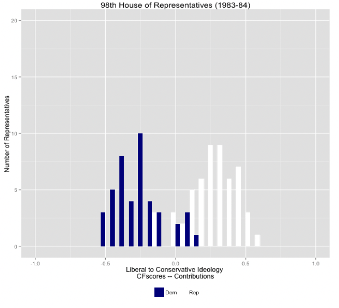
\includegraphics{images/Picture1.png} & 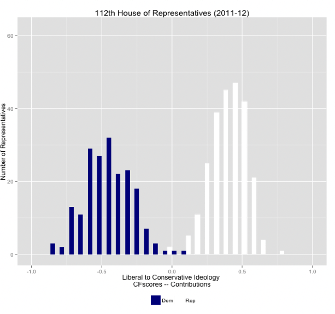
\includegraphics{images/Picture2.png} \\
    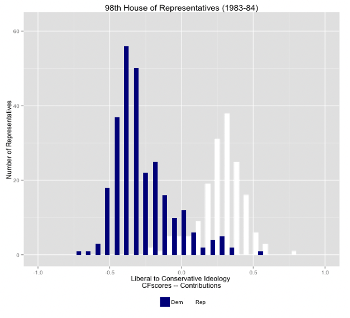
\includegraphics{images/Picture3.png} & 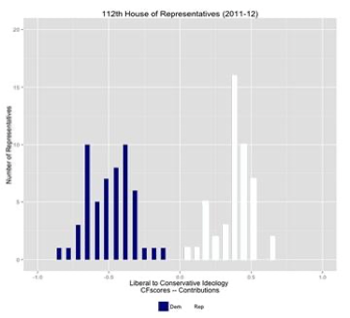
\includegraphics{images/Picture4.png} \\
    \end{tabular}
    \caption{ Construction of ideological distributions of the $98^{th}$ and $112^{th}$ House and Senate by Bonica and Rosenthal (2013)}
    \label{fig:my_label}
\end{figure}

\noindent consistent appearance of close elections in 1960 which had been relatively rare beforehand and according to \citeA{heltzelLaurin2020} occurred alongside increasing political polarization. Unfortunately, their data which is available for earlier time periods is not of a high enough frequency to utilize in a regression alongside variables influenced by the business cycle. Had monthly or quarterly data been available, it might have been able to shed more light on the larger D-R gap during the pre-Ronald Reagan years. The specific index of political polarization to be used in this analysis was originally detailed by \citeA{azzimonti2013} and will be described in Section 3. \par 





\section{Data}
Data is quarterly with a sampling period beginning at the start of Eisenhower’s second term and ending most of the way through Trump’s (1957:Q2 to 2020:Q2)\footnote{Quarters three and four in 2020 are excluded due to lack of availability for some variables.}. The single exception is polarization which begins with Reagan’s first term (1981:Q2 to 2020:Q2). Also, the data for oil price shocks is not discussed until Section 4 because of a lack of interpretability along with significant methodological complexity. \par

The measure utilized in this analysis for political polarization is an index created by \citeA{azzimonti2013} by categorizing search data from over 36,000 news sources from the database Factiva (by Dow Jones) for articles containing terms relating both to political polarization and to federal politics. The number of articles meeting the necessary criteria in a given time period was divided by the total number of articles published, and then normalized to an index based in 1990. Data originates from the Federal Reserve Bank of Philadelphia and is only available starting the first quarter of 1981. The index averaged 120.1 and 103.2 during Democrat and Republican presidencies respectively, a difference of 16.88\% ($p < 0.01$). Also, although not discussed here or in Table 1, the model in Section 4 uses first-differenced data for the political polarization index in order to maintain stationarity.\par

Cyclically adjusted Total Factor Productivity, measured here in percent change from a year before and collected from the FRB of St. Louis, was one of the strongest predictors of GDP growth rate in the subset of \citeauthor{blinderwatson2016}’s models that utilized data beginning in quarter two of 1949. Its growth rate in the full sampling period here averaged 1.001\% under Democratic presidents and 1.115\% under Republicans, an insignificant gap ($p = 0.782$). Excluding the pre-Reagan terms lowers the averages to 0.7488\% and 0.785\% respectively, also insignificant. \par

Financial sector disruptions downloaded from the FRB of St. Louis were measured using the Baa-Aaa yield spread in percentage points. The average spread was 0.286 percentage points higher under republicans ($p < 0.001$) for the full time period and 0.312 percentage points for the data including Reagan and onward. Although not discussed here or in Table 1, the model in section 4 utilizes first-differenced data for the Baa-Aaa yield spread in order to maintain stationarity. \par

The effective federal funds rate from the FRB of St. Louis is measured in percentage points. During the comprehensive data range there was an average of 4.107 \par 

\begin{landscape}
 % Table created by stargazer v.5.2.2 by Marek Hlavac, Harvard University. E-mail: hlavac at fas.harvard.edu
% Date and time: Tue, Nov 24, 2020 - 20:00:39
\begin{table}[!htbp] \centering 
  \caption{Descriptive Statistics} 
  \label{} 
\begin{tabular}{@{\extracolsep{5pt}} ccccccccc} 
\\[-1.8ex]\hline 
\hline \\[-1.8ex] 
& \multicolumn{4}{c}{Model 1 Data Range: 1957:Q2 to 2020:Q2} & \multicolumn{4}{c}{Models 2 and 3 Data Range: 1981:Q2 to 2020:Q2}\\
\hline \\[-1.8ex] 
 & Democrat & Republican & Difference & P-value & Democrat  & Republican  & Difference  & P-value  \\ 
\hline \\[-1.8ex] 
Total Factor Productivity (GR) & 1.002 & 1.115 & -0.1135 & 0.782 & 0.7488 & 0.7849 & -0.0362 & 0.94 \\ 
 & (0.313) & (0.263) &  &  & (0.389) & (0.279) &  &  \\ 
Baa-Aaa Spread (PP) & 0.8442 & 1.13 & -0.2859 & 2.97e-08 & 0.8804 & 1.192 & -0.3116 & 1.66e-06 \\ 
 & (0.0339) & (0.0366) &  &  & (0.0394) & (0.0486) &  &  \\ 
 Federal Funds Rate (PP) & 4.107 & 5.454 & -1.347 & 0.00304 & 2.652 & 5.47 & -2.818 & 2.12e-07 \\ 
 & (0.336) & (0.299) &  &  & (0.323) & (0.406) &  &  \\ 
Real GDP (GR) & 3.53 & 2.549 & 0.9814 & 0.00105 & 2.827 & 2.488 & 0.3384 & 0.303 \\ 
 & (0.198) & (0.22) &  &  & (0.206) & (0.254) &  &  \\ 
Political Polarization (Index) &  &  &  &  & 120.1 & 103.2 & 16.88 & 0.00378 \\ 
 &  &  &  &  & (4.68) & (3.29) &  &  \\
Defense Spending (GR) & 3.227 & 5.639 & -2.412 & 0.000967 & -0.3011 & 7.143 & -7.444 & 1.45e-22 \\ 
 & (0.589) & (0.415) &  &  & (0.428) & (0.483) &  &  \\ 
 Real GDP Per Capita (GR) & 2.422 & 1.486 & 0.9365 & 0.00125 & 1.844 & 1.562 & 0.2814 & 0.375 \\ 
 & (0.186) & (0.219) &  &  & (0.192) & (0.251) &  &  \\ 
Nonfarm Business Output (GR) & 3.99 & 2.695 & 1.295 & 0.000824 & 3.35 & 2.657 & 0.693 & 0.0975 \\ 
 & (0.243) & (0.295) &  &  & (0.261) & (0.323) &  &  \\ 
Industrial Production (GR) & 3.835 & 1.631 & 2.204 & 0.000293 & 2.752 & 1.339 & 1.413 & 0.0356 \\ 
 & (0.395) & (0.452) &  &  & (0.504) & (0.435) &  &  \\ 
Unemployment Rate (PP) & 5.84 & 6.072 & -0.2315 & 0.269 & 6.217 & 6.17 & 0.0473 & 0.872 \\ 
 & (0.156) & (0.138) &  &  & (0.227) & (0.184) &  &  \\ 
Output/hour (NFB)(GR) & 2.047 & 2.071 & -0.0236 & 0.912 & 1.717 & 2.034 & -0.3172 & 0.189 \\ 
 & (0.161) & (0.141) &  &  & (0.189) & (0.148) &  &  \\ 
Inflation PCED (PP) & 2.714 & 3.597 & -0.883 & 0.00422 & 1.62 & 3.088 & -1.468 & 1.85e-12 \\ 
 & (0.247) & (0.179) &  &  & (0.1) & (0.162) &  &  \\
\hline \\[-1.8ex] 
\singlespacing{ {\footnotesize Notes: Data from 2nd, 3rd, 6th, and 7th columns is in average value for numbers without parenthesis and standard error for numbers in parenthesis. Difference is equal to Democrat column value minus Republican column value. P-value columns are significance levels from two-sample t-tests of differences. GR denotes growth rate from a year ago in percentage points; PP denotes level in percentage points; NFB denotes non-farm business sector; PCED is the price deflator for personal consumption and GDP. Data from rows two through seven in Table 1 will not be included in the model nor discussed in-depth; rather, they are here both to provide more context and because they were included in a similar table of descriptive statistics by Blinder and Watson (2016).}}
\end{tabular} 
\end{table} 
\end{landscape} 

\noindent and 5.454 percentage points for Democrats and Republicans respectively, with the difference between the two being significant ($p < 0.01$). The shortened data range saw an even larger difference at 2.818 percentage points ($p < 0.001$) with the average under Democrats falling to 2.652 percentage points. This decrease can largely be attributed to the extreme expansionary monetary policy occurring during the Obama administration taking up a larger percentage of the shortened sample.\par

Presidential party is measured using a dummy variable (1 = Democrat and 0 = Republican) with the first financial quarter after an election year being attributed to the previous president in order to account for an assumed lag effect of at least one period, as was done in \citeA{blinderwatson2016}\footnote{It should be noted Blinder and Watson found that alternative lag and lead effects up to a period of four all lead to smaller D-R gaps.}. The full sampling period contains almost sixteen presidential terms, seven under Democrats and eight full terms under Republicans plus the Trump administration up to the second quarter of 2020. The shorter sampling period beginning with Reagan contains a total of thirteen terms, five under Democrats and seven under Republicans plus part of Trump's. \par

Real GDP growth rate from the FRB of St. Louis is measured in percentage point change from a year beforehand. Over the full sample period, the average real GDP growth rate was 3.53\% for Democrats and 2.549\% for Republicans, meaning a 0.981 percentage point D-R gap ($p < 0.01$). This is far less than \citeauthor{blinderwatson2016}’s findings of a 1.79 percentage point gap, with the decrease accounted for by the addition of Obama’s second term and most of Trump’s, as well as the removal of Truman’s second and Eisenhower’s first terms. The removal of the aforementioned two terms was also performed by \citeauthor{blinderwatson2016} in their final models and will be discussed in Section 4 in reference to defense spending. The difference in values for the shortened data range is much smaller at 0.338 percentage points and insignificant ($p = 0.303$). This decrease in significance is understandable given the roughly 38\% decrease in sample size. However, the fact that the magnitude of the difference also changed so much despite a still hefty remaining sample size of 39 years (156 quarters) points toward the possibility of the D-R gap potentially being a figment of the past. Also, although not discussed here or in Table 1, the model in section 4 uses first-differenced data for real GDP growth rate in order to maintain stationarity.


\section{Methodology}
The model takes the price of oil as the crude petroleum component of the producer price index and creates a variable measuring price at time t relative to its maximum value over the previous 3 years \cite{hamilton2003}. Here, $P_t$ denotes the final variable to be used in the model, $O_t$ denotes curent price of oil and $O_{t-12:t-1}^{Max}$ is the greatest value of $O_t$ over the previous 12 quarters. Note that by taking the maximum of either zero or the second term, this measure presumes that only price increases are relevant and completely omits decreases.
\[P_t = max(0, 100*ln(\frac{O_t}{O_{t-12:t-1}^{Max}})\]

In their original article, \citeA{blinderwatson2016} attempted to include a variable for defense spending shocks in their model, but the one utilized \cite{ramey2011} only led to one significant shock during the Korean war. Because of this, they opted to account for higher defense spending by Democrats by removing Truman’s second and Eisenhower’s first term rather than including a relevant variable in their model. The addition to the data-set here does not show a defense spending shock similar in size to the Korean war, so rather than include \citeauthor{ramey2011}’s variable this model will also utilize a sample beginning with Eisenhower’s second term (1957:Q2 to 2020:Q2) despite all data being available as early as 1954. \par

With the exception of oil and defense spending, the implementations of all other variables are the same as described in Section III. Three models will be created, the first (1) utilizing the full post-Korean War time period (1957:Q2 to 2020:Q2) and the second (2) and third (3) being limited to Reagan's election and later (1981:Q2 to 2020:Q2). In order of the Cholesky decomposition in the model, variable denotations include “OIL” for the computed positive oil shocks, “TFP” for total factor productivity, “BA” for the Baa-Aaa bond yield spread, “FED” for the effective federal funds rate, “P” for the dummy variable on presidential party, and “GDP” for real gross domestic product growth rate. Model 3 also includes “POL” which denotes the political polarization index, and is placed first in the Cholesky Decomposition ordering, although relevant findings are robust to multiple orderings. It is designated as the most exogenous variable because of how slowly cultural phenomena tend to change over time. Model 2 exists in order to facilitate analysis of the other variables within the confines of POL's shortened time-span, thereby allowing for indirect comparison between Models 1 and 3. Lag values of six, two and twelve respectively have been chosen through AIC tests with twelve being the maximum allowed. All three Vector Autoregression (VAR) models are shown below in matrix form with $\alpha_t$ as the Cholesky Decomposition matrices.
\begin{align}
\alpha_ty_t = \beta_0 + \sum_{i=1}^6\gamma_iy_{t-i} + \epsilon_t\\
\alpha_ty_t = \beta_0 + \sum_{i=1}^2\gamma_iy_{t-i} + \epsilon_t\\
\alpha_ty_t = \beta_0 + \sum_{i=1}^{12}\gamma_iy_{t-i} + \epsilon_t
\end{align}



\section{Results}
For Model 1 containing the full post-Korea time-span, the only variables that fail to exhibit significant Granger causality are total factor productivity and the presidential dummy, although both are somewhat close ($P < 0.15$). Exact values for each variable can be found in Table 2. \citeA{blinderwatson2016} did not discuss Granger causality explicitly, but it is very likely that they found different results. The extent of their D-R gap was far larger (1.79 versus 0.981 percentage points) which is attributable to the change in sampling period. As seen in Table 3, after 8 time periods presidential party accounts for the smallest amount of the variance in GDP growth rate at only 2.4\%. The Baa-Aaa yield spread and the federal funds rate are the strongest predictors at 14.1\% and 14.3\% respectively, while 60.9\% of the variance in GDP is still left unexplained for \par 

 \begin{table}[!htbp] \centering 
  \caption{Granger Causality} 
  \label{} 
\begin{tabular}{@{\extracolsep{1pt}} ccccccccccc} 
\\[-1.8ex]\hline 
\hline \\[-1.8ex]
& \multicolumn{2}{c}{Model 1} & \multicolumn{2}{c}{Model 2} \multicolumn{2}{c}{Model 3}\\
\hline \\[-1.8ex]
& F(30, 1260) & P-value & F(10, 852) & P-value & F(72, 420) & P-value\\
\hline \\[-1.8ex] 
POL & & & & & 1.550 & 0.005\\
OIL & 2.651 & 0.001 & 1.633 & 0.093 & 1.726 & 0.001\\
TFP & 1.315 & 0.120 & 0.821 & 0.609 & 0.712 & 0.940\\
BA & 2.171 & 0.001 & 1.880 & 0.044 & 1.655 & 0.001\\
FED & 3.589 & 0.001 & 2.809 & 0.002 & 1.355 & 0.037\\
P & 1.337 & 0.106 & 0.888 & 0.544 & 0.638 & 0.990\\
GDP & 1.933 & 0.002 & 1.506 & 0.132 & 1.760 & 0.001\\
\hline \\[-1.8ex] 
\end{tabular} 
\end{table}

\noindent by the more exogenous predictors. The impulse response function for effect of the presidential dummy on GDP growth as well as its cumulative counterpart are both insignificant but show a trend favoring Democrats (Figure 2). \par

Model 2, which utilizes the shorter time period without the polarization variable, shows multiple changes in Granger causality. In comparison to Model 1, Oil price shocks and GDP growth rate become insignificant ($p = 0.093$ and $p = 0.132$ respectively) in their Granger causality while total factor productivity and the presidential party variable become even less significant than before. The explanatory power of every variable goes down to some extent due to the decrease in sample size, leaving only 22.8\% of the variance in GDP explained after eight time periods in contrast with 39.1\% in Model 1. Figure 3 shows an insignificant impulse response function still with a directional trend favoring a Democrat taking office. \par 

The third model is the most interesting with its inclusion of the political polarization index. First off is that oil price shocks and GDP growth rate once again gain significant values for Granger causality ($p < 0.001$ for both) while total factor productivity and the presidential party variable once again lose even more significance ($p = 0.940$ and $0.990$ respectively). Also of interest is that the new political polarization index is significant ($p < 0.01$). The variance decomposition of GDP in Table 5 shows this model's strength by the fact that only 42.3\% of the variance in GDP is left unaccounted for by the other variables after eight time periods. This is a large improvement over Model 1's value of 60.9\% despite the hefty decrease in sample size as well as from Model 2's value \par  

% Table created by stargazer v.5.2.2 by Marek Hlavac, Harvard University. E-mail: hlavac at fas.harvard.edu
% Date and time: Wed, Nov 25, 2020 - 13:50:09
\begin{table}[!htbp] \centering 
  \caption{Model 1's Variance Decomposition of GDP} 
  \label{} 
\begin{tabular}{@{\extracolsep{5pt}} ccccccc} 
\\[-1.8ex]\hline 
\hline \\[-1.8ex] 
Periods Ahead & OIL & TFP & BA & FED & P & GDP \\ 
\hline \\[-1.8ex] 
1&$0.002$ & $0.009$ & $0.056$ & $0.030$ & $0.007$ & $0.896$ \\ 
2&$0.003$ & $0.008$ & $0.108$ & $0.036$ & $0.011$ & $0.835$ \\ 
3&$0.003$ & $0.011$ & $0.113$ & $0.061$ & $0.027$ & $0.784$ \\ 
4&$0.010$ & $0.024$ & $0.108$ & $0.089$ & $0.025$ & $0.744$ \\ 
5&$0.024$ & $0.036$ & $0.113$ & $0.119$ & $0.020$ & $0.687$ \\ 
6&$0.023$ & $0.040$ & $0.130$ & $0.150$ & $0.022$ & $0.635$ \\ 
7&$0.035$ & $0.041$ & $0.137$ & $0.144$ & $0.023$ & $0.619$ \\ 
8&$0.040$ & $0.043$ & $0.141$ & $0.143$ & $0.024$ & $0.609$ \\ 
\hline \\[-1.8ex] 
\end{tabular} 
\end{table} 
% Table created by stargazer v.5.2.2 by Marek Hlavac, Harvard University. E-mail: hlavac at fas.harvard.edu
% Date and time: Wed, Nov 25, 2020 - 22:29:24
\begin{table}[!htbp] \centering 
  \caption{Model 2's Variance Decomposition of GDP} 
  \label{} 
\begin{tabular}{@{\extracolsep{5pt}} ccccccc} 
\\[-1.8ex]\hline 
\hline \\[-1.8ex] 
Periods Ahead & OIL & TFP & BA & FED & P & GDP \\
\hline \\[-1.8ex] 
1&$0.001$ & $0.033$ & $0.085$ & $0.034$ & $0.0004$ & $0.847$ \\ 
2&$0.001$ & $0.027$ & $0.113$ & $0.041$ & $0.002$ & $0.816$ \\ 
3&$0.004$ & $0.026$ & $0.111$ & $0.048$ & $0.005$ & $0.806$ \\ 
4&$0.011$ & $0.025$ & $0.108$ & $0.055$ & $0.007$ & $0.794$ \\ 
5&$0.013$ & $0.025$ & $0.113$ & $0.055$ & $0.007$ & $0.786$ \\ 
6&$0.013$ & $0.025$ & $0.120$ & $0.055$ & $0.008$ & $0.779$ \\ 
7&$0.013$ & $0.025$ & $0.123$ & $0.056$ & $0.008$ & $0.774$ \\ 
8&$0.014$ & $0.025$ & $0.125$ & $0.055$ & $0.009$ & $0.772$ \\ 
\hline \\[-1.8ex] 
\end{tabular} 
\end{table} 
% Table created by stargazer v.5.2.2 by Marek Hlavac, Harvard University. E-mail: hlavac at fas.harvard.edu
% Date and time: Wed, Nov 25, 2020 - 22:38:04
\begin{table}[!htbp] \centering 
  \caption{Model 3's Variance Decomposition of GDP} 
  \label{} 
\begin{tabular}{@{\extracolsep{5pt}} cccccccc} 
\\[-1.8ex]\hline 
\hline \\[-1.8ex] 
Periods Ahead & POL & OIL & TFP & BA & FED & P & GDP \\
\hline \\[-1.8ex] 
1 & $0.033$ & $0.025$ & $0.121$ & $0.100$ & $0.062$ & $0.013$ & $0.646$ \\ 
2 & $0.162$ & $0.033$ & $0.124$ & $0.128$ & $0.044$ & $0.016$ & $0.492$ \\ 
3 & $0.185$ & $0.030$ & $0.144$ & $0.134$ & $0.044$ & $0.015$ & $0.449$ \\ 
4 & $0.234$ & $0.030$ & $0.142$ & $0.129$ & $0.043$ & $0.015$ & $0.407$ \\ 
5 & $0.196$ & $0.025$ & $0.167$ & $0.112$ & $0.038$ & $0.014$ & $0.447$ \\ 
6 & $0.182$ & $0.024$ & $0.169$ & $0.112$ & $0.036$ & $0.017$ & $0.460$ \\ 
7 & $0.183$ & $0.025$ & $0.172$ & $0.124$ & $0.038$ & $0.017$ & $0.442$ \\ 
8 & $0.187$ & $0.025$ & $0.171$ & $0.126$ & $0.049$ & $0.020$ & $0.423$ \\ 
\hline \\[-1.8ex] 
\end{tabular} 
\end{table} 

\begin{figure}
    \centering
    \begin{tabular}{cc}
    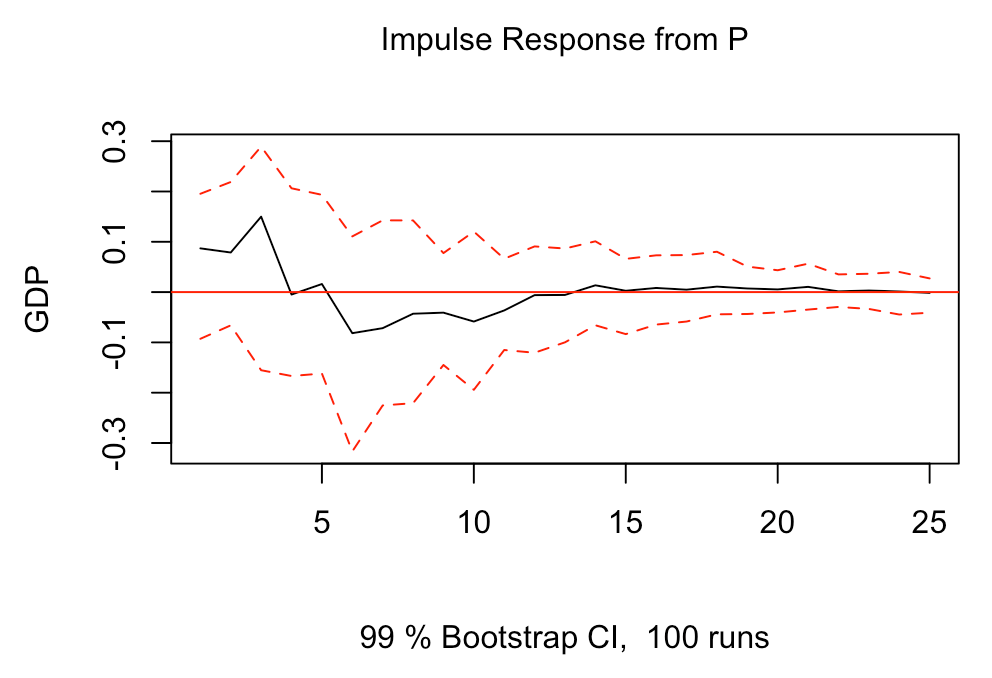
\includegraphics[scale = .39]{model1/Screen Shot 2020-11-26 at 12.47.31 AM.png} & 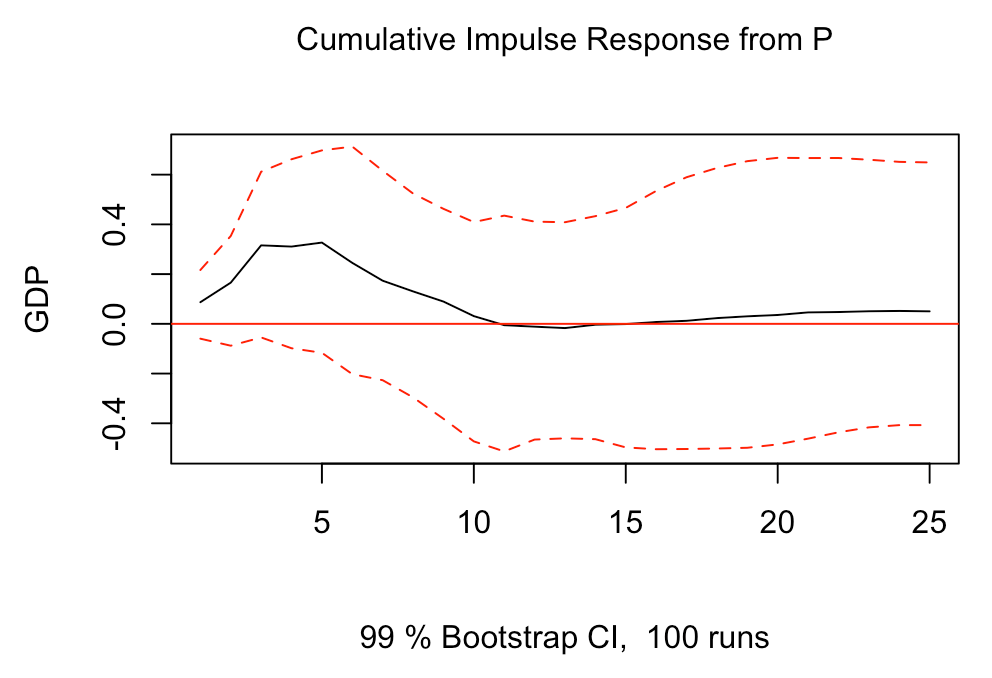
\includegraphics[scale = .39]{model1/Screen Shot 2020-11-26 at 12.47.36 AM.png} \\
    \end{tabular}
    \caption{Model 1's impulse response function for effect of a shock to the presidential party dummy variable (AKA a Democrat taking office) on GDP growth rate}
    \label{fig:my_label}
\end{figure}
\begin{figure}
    \centering
    \begin{tabular}{cc}
    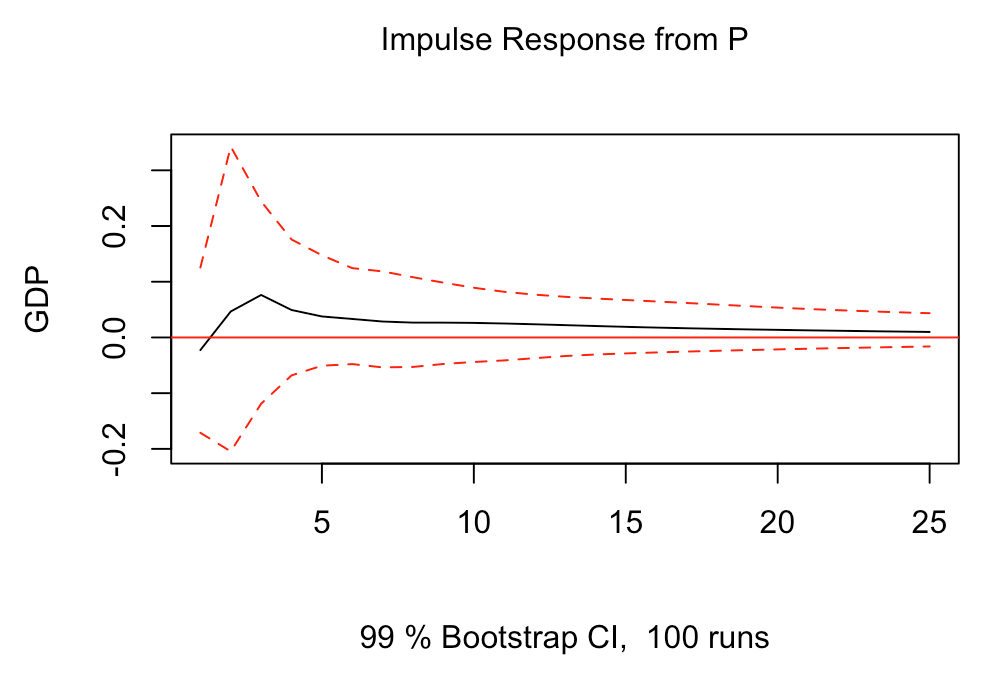
\includegraphics[scale = .39]{model2/Screen Shot 2020-11-26 at 12.53.30 AM.png} & 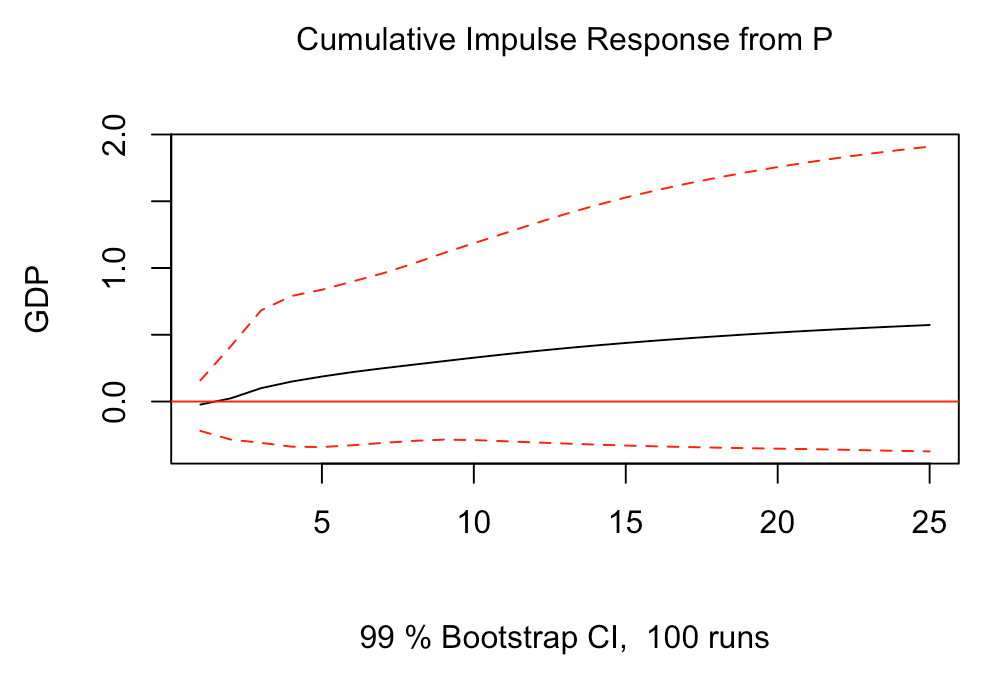
\includegraphics[scale = .39]{model2/Screen Shot 2020-11-26 at 12.53.41 AM.png} \\
    \end{tabular}
    \caption{Model 2's impulse response function for effect of a shock to the presidential party dummy variable (AKA a Democrat taking office) on GDP growth rate}
    \label{fig:my_label}
\end{figure}
\begin{figure}
    \centering
    \begin{tabular}{cc}
    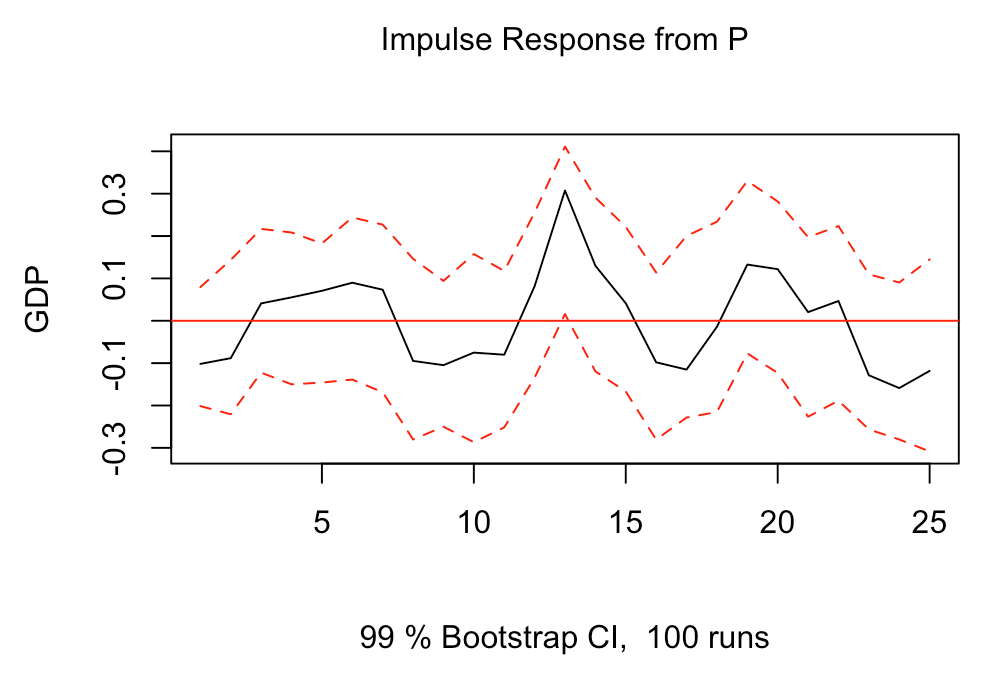
\includegraphics[scale = .39]{model3/P/Screen Shot 2020-11-26 at 12.59.22 AM.png} & 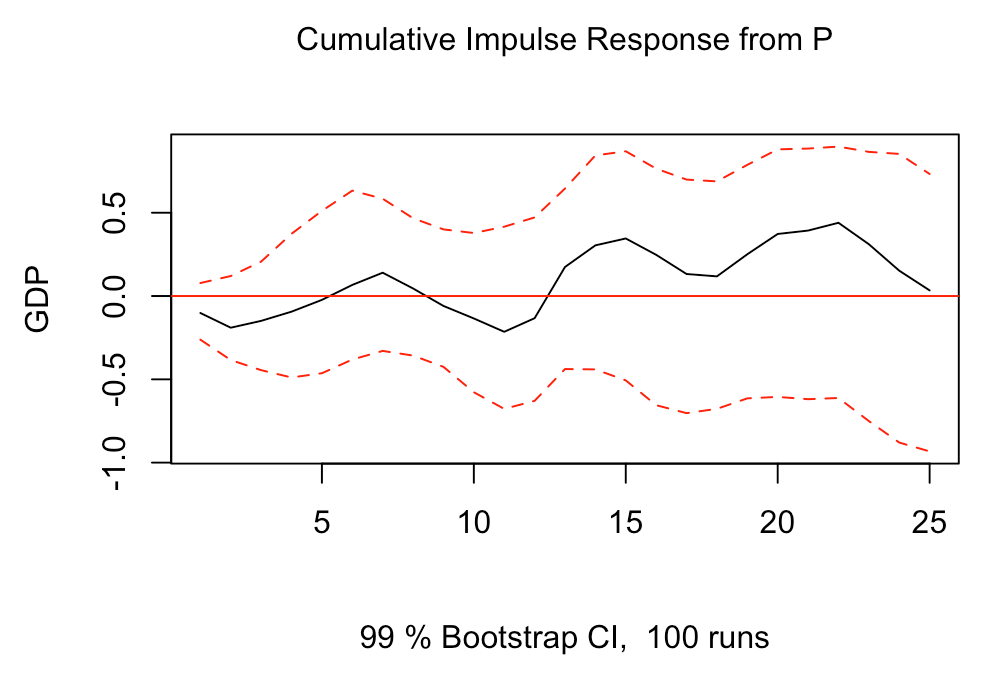
\includegraphics[scale = .39]{model3/P/Screen Shot 2020-11-26 at 12.59.36 AM.png} \\
    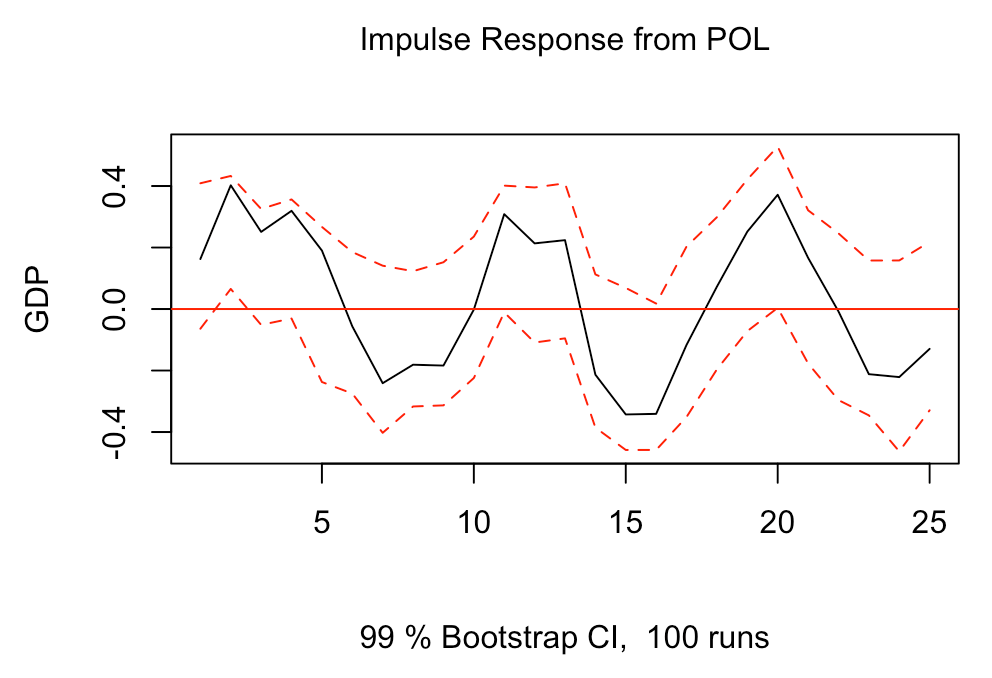
\includegraphics[scale = .39]{model3/POL/Screen Shot 2020-11-26 at 1.00.25 AM.png} & 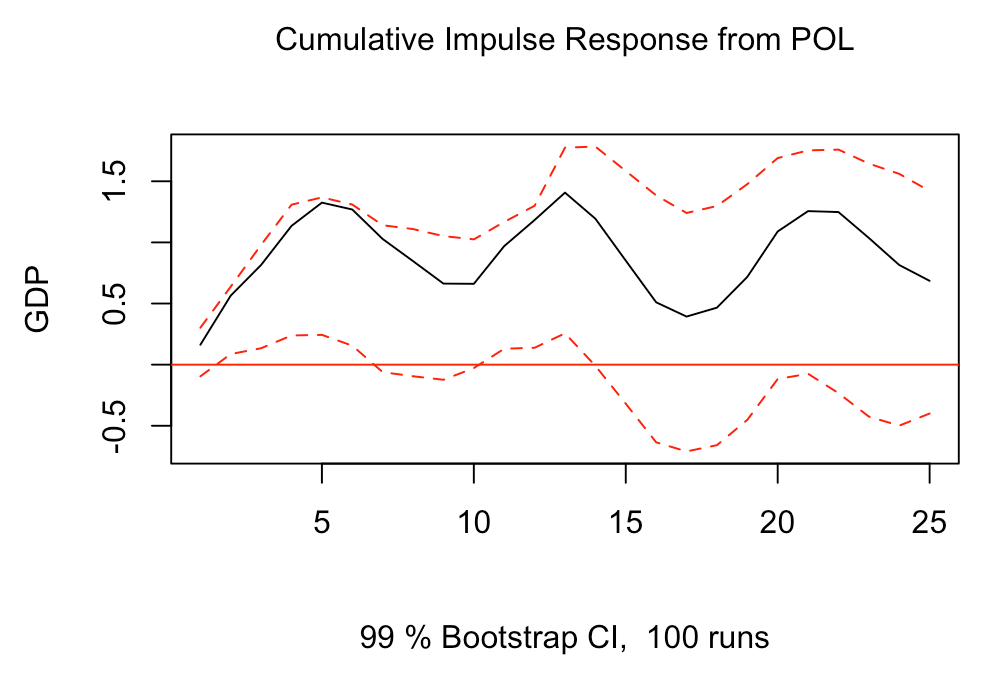
\includegraphics[scale = .39]{model3/POL/Screen Shot 2020-11-26 at 1.00.35 AM.png}
    \end{tabular}
    \caption{Model 3's impulse response functions for the effect of a shock to the presidential party dummy variable (AKA a Democrat taking office) as well as to the political polarization index (AKA a 1 point increase in the index) on GDP growth rate}
    \label{fig:my_label}
\end{figure}

\newpage
\begin{figure}
    \centering
    \begin{tabular}{cc}
    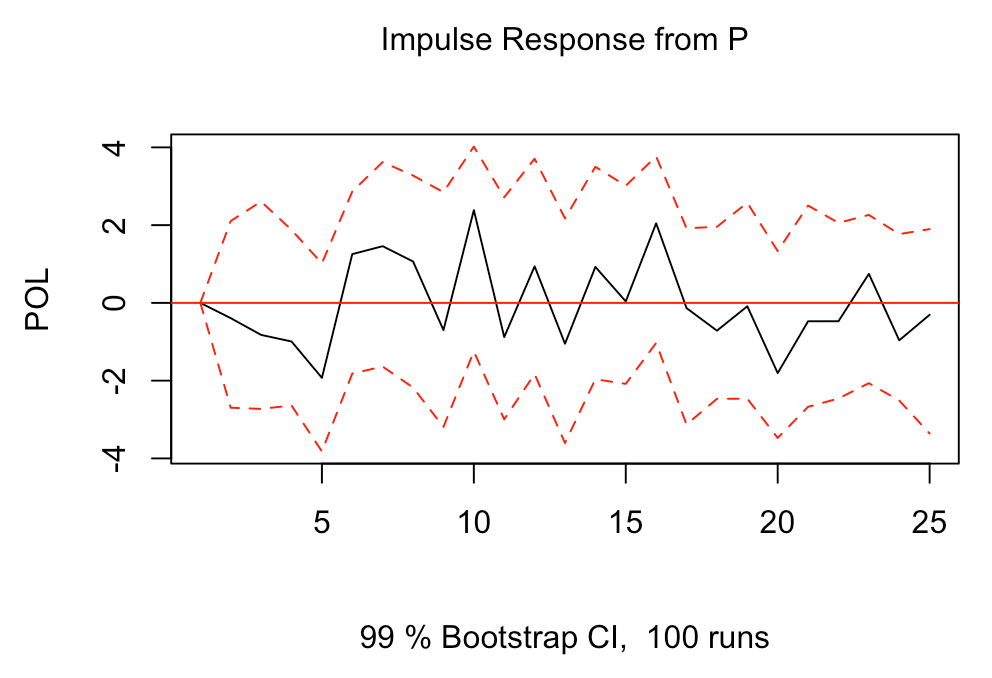
\includegraphics[scale = .39]{model3/extra?/Screen Shot 2020-11-26 at 3.17.10 PM.png} & 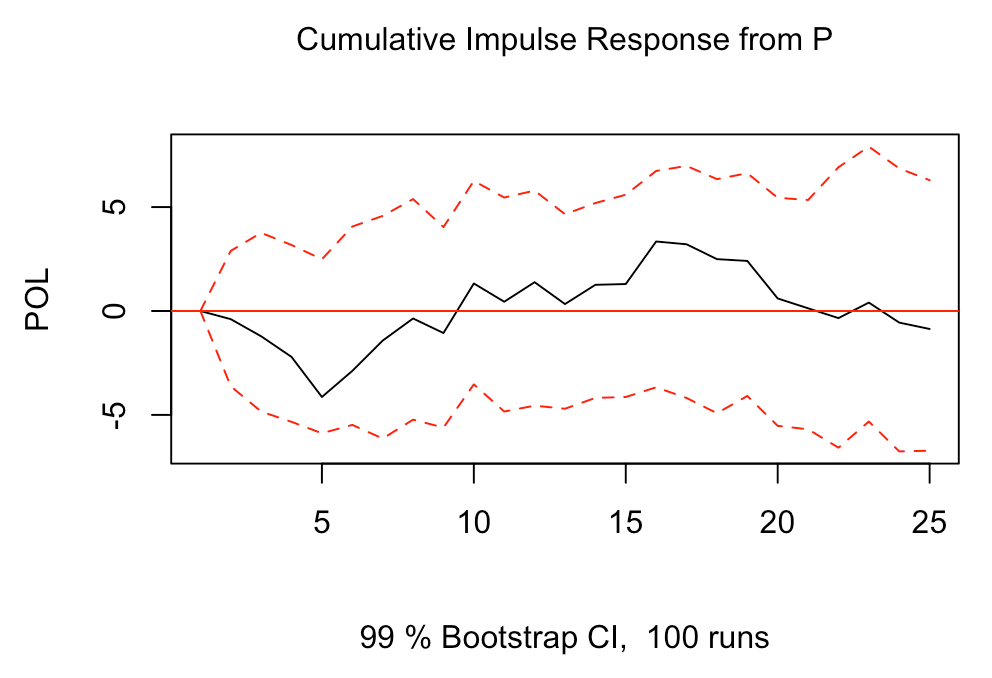
\includegraphics[scale = .39]{model3/extra?/Screen Shot 2020-11-26 at 3.17.37 PM.png} \\
    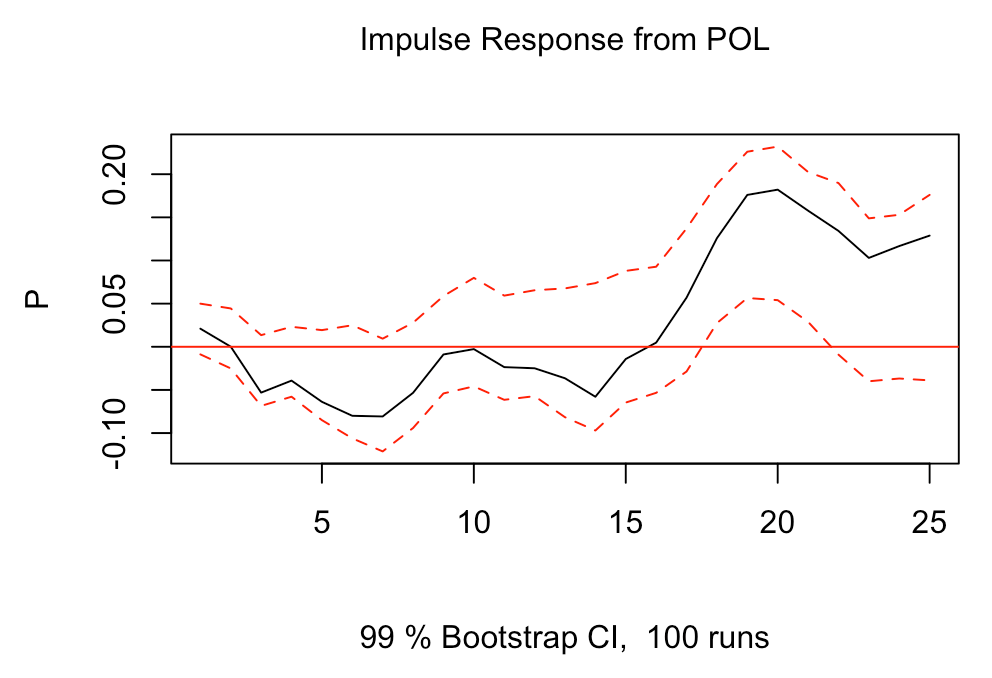
\includegraphics[scale = .39]{model3/extra?/Screen Shot 2020-11-26 at 3.19.06 PM.png} & 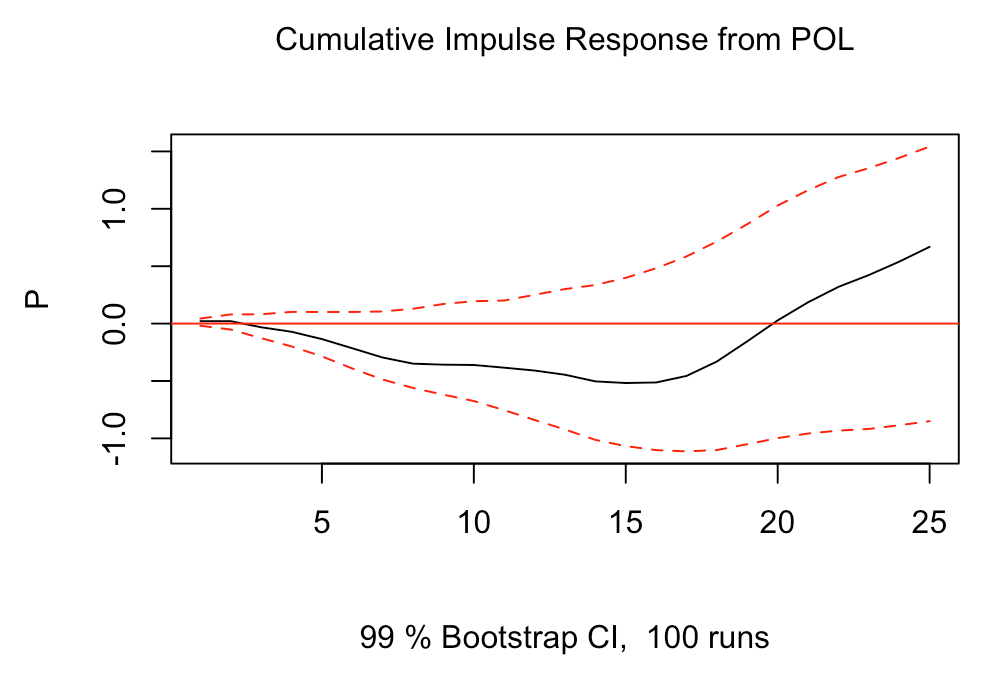
\includegraphics[scale = .39]{model3/extra?/Screen Shot 2020-11-26 at 3.19.55 PM.png}
    \end{tabular}
    \caption{Effect of shock to presidential party (AKA a Democrat taking office) on polarization is top row and effect of a 1 point increase in the polarization index on presidential party variable is bottom row.}
    \label{fig:my_label}
\end{figure}


\noindent of 77.2\%. Curiously, the amount of variance in GDP explained by total factor productivity ascended here to 17.1\% from 4.3\% in Model 1 and 2.5\% in Model 2 despite its low significance in the aforementioned Granger causality test. This brings total factor productivity ahead of the Baa-Aaa yield spread, the previous leader which fluctuates between 12.5\% and 14.1\% throughout the three models. However, the most powerful variable is the political polarization index with a value of 0.187 meaning that 18.7\% of the variance in real GDP growth rate is accounted for by shocks to polarization. In Figure 4 the impulse response function of the presidential party dummy on GDP growth is still insignificant like in the other models but no longer shows the consistent trend favoring a Democrat taking office. Figure 4 also depicts the impulse response of the political polarization index on GDP, with only one time period being significant in the regular graph. On the cumulative IRF, multiple periods on two separate intervals are significant\footnote{The expected value for the impulse response function shown is very close to the 99\% upper-bound, and would actually surpass the upper bound if a 95\% confidence interval were used. Although rare, this is theoretically possible \cite{hoekstra2015}. The same effect can be seen in the bottom left of Figure 5.}. The data here implies that a random shock increase in polarization elicits an increased GDP growth rate, which goes contrary to the theoretical expectation and previous experimental data specified in Sections 1 and 2. Finally, positive shocks to polarization have a bit of predictive power on presidential party in the direction of getting Democrats elected, albeit with a very delayed (roughly five year) effect. There is no significant effect to be found in the opposite direction, as can be seen in Figure 5. \par 




\section{Conclusion}
This paper downplays the findings of a persistent D-R gap by \citeA{blinderwatson2016} through a data update. It could be the case that the highly significant pre-Reagan values are a figment of the past, but it might also be true that the Obama-Trump era is the anomaly. The latter possibility is especially interesting given that it could stem from circumstances specific to the aftermath of the 2008 financial crisis. Future data collection will be necessary to determine whether this trend of the D-R gap decreasing over time continues. However, this paper's analysis is comparatively lacking both in regards to statistical interpretation methods and in many cases the use of simpler variables where \citeauthor{blinderwatson2016} derived more complicated measures of shocks. \par

Positive shocks to polarization are highly predictive of positive GDP growth despite theoretical predictions and previous experimental data in the reverse direction \cite{azzimonti2013, azzimontiTalbert2014, bakerBloomDavis2016}. Future research will be needed to thoroughly explain the discrepancy between the results here and those of \citeauthor{azzimonti2013}. Initial ideas include the addition here of data points from after 2013, differences in variables included between models, and the differing methods for measurement of GDP growth (\citeauthor{azzimonti2013} uses first-differenced natural log of quarterly GDP while this analysis utilizes first-differenced quarterly GDP measured in percent change from a year beforehand). Either way, polarization's effect on growth is likely attributable to some as-of-yet unexplored byproduct of the way political polarization affects or aligns with either consumer and producer behavior or legislation, and this analysis would benefit from research bridging that gap. \par
Finally, the facts that (I) polarization is higher when a Democrat is president, (II) its inclusion decreases the predictive power of presidential party on GDP growth, (III) it has some predictive power on presidential party and (IV) it is the best predictor of GDP growth in the analysis all together strongly point towards polarization being a mediating factor of the D-R gap. However, the D-R gap was already diminished into insignificance in the shortened range of Models 2 and 3 meaning that data on earlier time periods is needed before a definitive statement can be made.

\newpage
\bibliographystyle{apacite}
\bibliography{bib}
%\printbibliography

\end{document}
